% file: HTH-automaton.tex

\documentclass[tikz]{standalone}
\usetikzlibrary{automata, positioning, arrows.meta}

\begin{document}
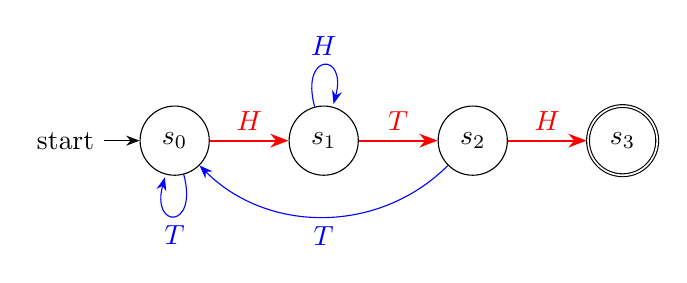
\begin{tikzpicture}[->, >=Stealth, auto, 
  	forward/.style = {thick, red},
	backward/.style = {blue}]
  \node[state, initial] (s0) {$s_0$};
  \node[state, right = of s0] (s1) {$s_1$};
  \node[state, right = of s1] (s2) {$s_2$};
  \node[state, accepting, right = of s2] (s3) {$s_3$};

  \path (s0) edge[forward] node {$H$} (s1)
	     edge[backward, loop below] node {$T$} ()
	(s1) edge[forward] node {$T$} (s2)
	     edge[backward, loop above] node {$H$} (s1)
	(s2) edge[forward] node {$H$} (s3)
	     edge[backward, bend left = 45] node {$T$} (s0);
\end{tikzpicture}
\end{document}
